\section{Architecture}
\label{sec:architecture}

However, PAWS has faced ongoing deployment challenges such as limited coverage and most importantly due to home user sharing patterns. We have noticed that the PAWS routers were always not available mainly due to home users plugging off the PAWS router from the Ethernet socket of the home router and reusing the socket for their own use or because they did not want to share their Internet connection with the others for certain periods of the day or for other reasons such as economic constraints placed on home users in underprivileged areas where they are forced to conserve energy by turning off the routers at nights. Figure \ref{fig:paws-avail} presents a six-month view of the PAWS routers status (available/unavailable) logs demonstrating that not a single router was available continuously over the entire duration. These observed user behaviors have become serious challenges for the successful adoption of PAWS. 

\begin{figure}[h]
\begin{center}
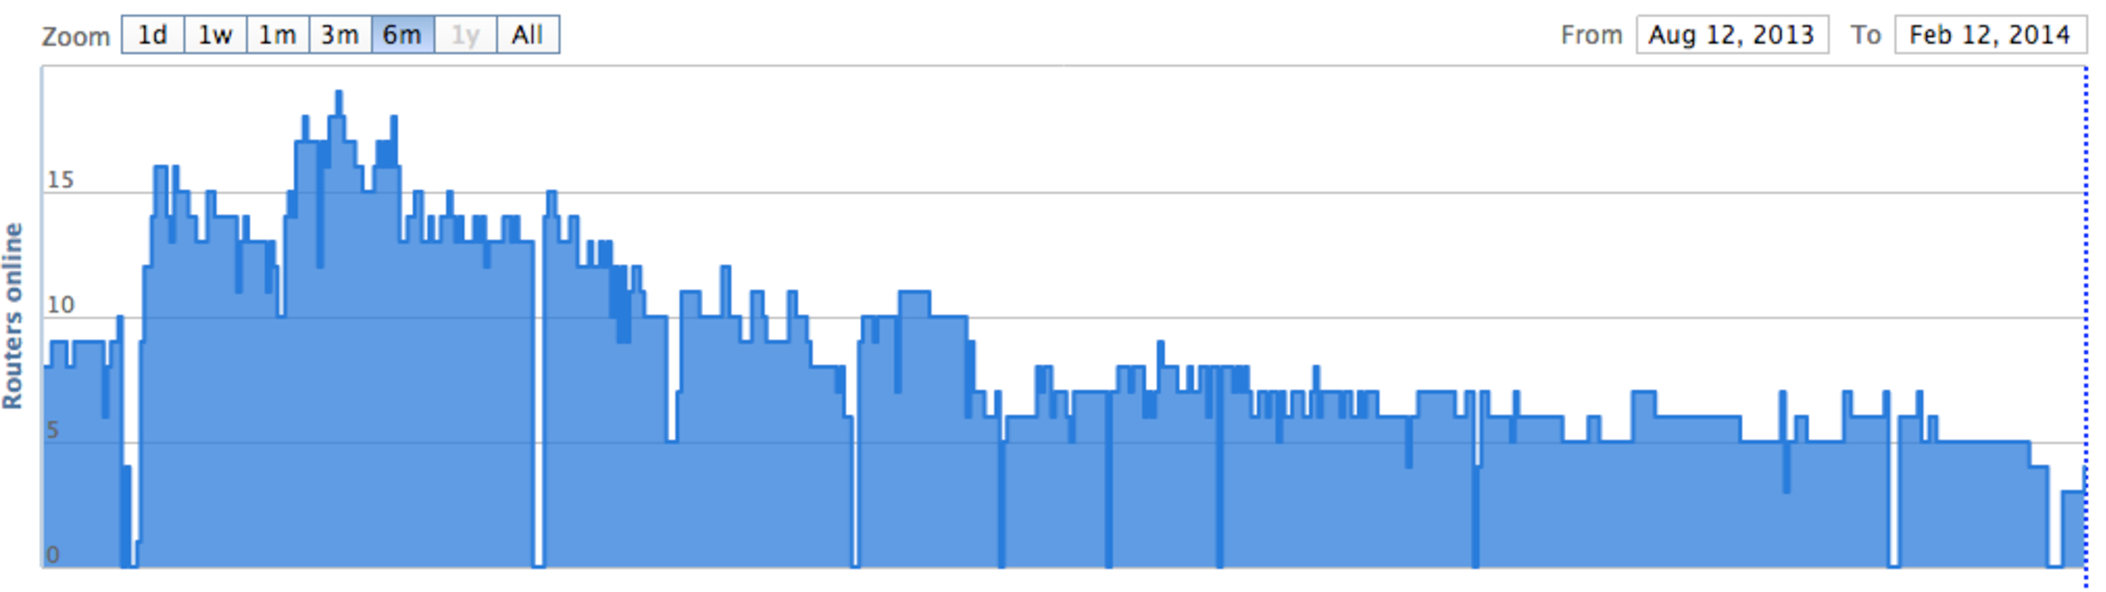
\includegraphics[width=1\linewidth]{paws-avail.pdf}  
\caption{PAWS routers availability.}
\label{fig:paws-avail}
\end{center}
\end{figure}

The underlying problem with PAWS or any crowd-shared network (such as FON) is that they serve as single point of Internet access to users within the coverage of the wireless router and hence have no provision to extend the coverage or to provide any redundancy during unavailability of the routers which is mainly due to the sharerÕs sharing tendencies or policies. A potential solution to these problems would be to extend the PAWS network as a crowd-shared mesh network. Such a network would allow home broadband users to share part of their own broadband connection to the public for free while also connected to each other as a wireless mesh providing extended coverage. This also offers network redundancy to the Internet backhaul even when some sharers decide not to share their backhaul Internet connection for certain periods of time. 

In this paper, we explore the potential benefits of enabling PAWS or any crowd-shared wireless network as a crowd-shared wireless mesh network. Our paper provides the following contributions:
%\begin{enumerate}
%\end{enumerate}

